\begin{enumerate}
\item
\begin{align}
\begin{split}
\myvec{1 & 1 }\vec{x}&=14
\\
\myvec{1 & -1 }\vec{x}&=4
\end{split}
\end{align}
The above equations can be expressed as the matrix equation
\begin{align}
\myvec{1 & 1\\1 & -1} \vec{x} = \myvec{14\\4}
\end{align}
%
The augmented matrix for the above equation is row reduced as follows
\begin{align}
\myvec{1 & 1 & 14\\1 & -1 & 4} 
\xleftrightarrow {R_2\leftarrow R_2 -R_1}\myvec{1 & \ 1 & 14 \\0 & -2 & -10 }
\\
%\myvec{1 & 1 & 14\\0 & -2 & -10} 
\xleftrightarrow {R_1\leftarrow R_1 -R_2/-2}\myvec{1 & \ 0 & 9 \\0 & -2 & -10 }
\\
%\myvec{1 & 0 & 9\\0 & -2 & -10} 
\xleftrightarrow {R_2\leftarrow R_2/-2}\myvec{1 & \ 0 & 9 \\0 & 1 & 5 }
\end{align}
%
As left part is converted into identity matrix the intersection vector is \myvec{9\\5} which is plotted in Fig.     \ref{linform/10/ab/fig:INTERSECTING LINES}
%
\begin{figure}[ht!]
    \centering
    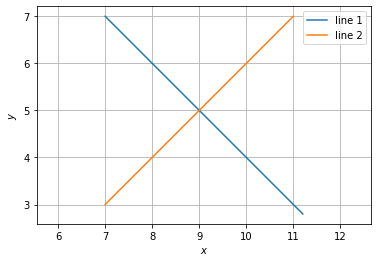
\includegraphics[width=\columnwidth]{solutions/su2021/2/10/ab/figure1.png}
    \caption{INTERSECTING LINES}
    \label{linform/10/ab/fig:INTERSECTING LINES}
\end{figure} 
\item
\begin{align}
\begin{split}
\myvec{1 & -1 }\vec{x}&=3  
\\
\myvec{\frac{1}{3} & \frac{1}{2}}\vec{x}&=6
\end{split}
\end{align}
The above equations can be expressed as the matrix equation
\begin{align}
\myvec{1 & -1\\\frac{1}{3} & \frac{1}{2}} \vec{x} = \myvec{3\\6}
\end{align}
%
The augmented matrix for the above equation is row reduced as follows
\begin{align}
\myvec{1 & -1 & 3\\\frac{1}{3} &\frac{1}{2} & 6 }
\xleftrightarrow {R_2\leftarrow R_2-R_1/3}\myvec{1 & -1 & 3 \\0 & \frac{5}{6} & 5}
\\
%\myvec{1 & -1 & 3\\0 &\frac{5}{6} & 5}
\xleftrightarrow {R_2\leftarrow R_2/5}\myvec{1 & -1 & 3 \\0 & \frac{1}{6} & 1}
\\
%\myvec{1 & -1 & 3\\0 &\frac{1}{6} & 1 }
\xleftrightarrow {R_2\leftarrow 6R_2}\myvec{1 & -1 & 3 \\0 & 1 & 6}
\\
%\myvec{1 & -1 & 3\\0 &1 & 6 }
\xleftrightarrow {R_2\leftarrow R_2+R_1}\myvec{1 & 0 & 9 \\0 & 1 & 6}
\end{align}
%
As left part is converted into identity matrix the intersection vector is \myvec{9\\6}
which is plotted in Fig.     \ref{linform/10/ab/fig:INTERSECTING LINES2}.
\begin{figure}[!ht]
    \centering
   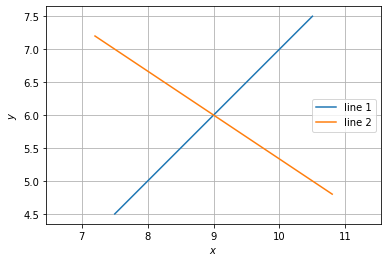
\includegraphics[width=\columnwidth]{solutions/su2021/2/10/ab/figure2.png}
    \caption{INTERSECTING LINES}
    \label{linform/10/ab/fig:INTERSECTING LINES2}
\end{figure}    
